\documentclass[11pt, a4paper]{article}
\usepackage{pdfpages}
\usepackage{parallel}
\usepackage[T2A]{fontenc}
%\usepackage{ucs}
\usepackage[utf8]{inputenc}
\usepackage[english,russian]{babel}
\usepackage{hyperref}
\usepackage{rotating}
\usepackage[inner=2cm,top=1.8cm,outer=2cm,bottom=2.3cm,nohead]{geometry}
%\usepackage{listings}
\usepackage{graphicx}
\usepackage{wrapfig}
\usepackage{longtable}
\usepackage{indentfirst}
\usepackage{array}
\usepackage{tikzsymbols}
\usepackage{soul}
\usepackage[ruled,vlined]{algorithm2e}
\usepackage{qrcode}
\counterwithout{figure}{section} 

\usepackage{url}
\makeatletter
\g@addto@macro{\UrlBreaks}{\UrlOrds}
\makeatother

\newcolumntype{P}[1]{>{\raggedright\arraybackslash}p{#1}}
\frenchspacing
%\usepackage{fixltx2e} %text sub- and superscripts
\usepackage{icomma} % коскі ў матэматычным рэжыме
%\PreloadUnicodePage{4}

\newcommand{\longpage}{\enlargethispage{\baselineskip}}
\newcommand{\shortpage}{\enlargethispage{-\baselineskip}}

\def\switchlang#1{\expandafter\csname switchlang#1\endcsname}
\def\switchlangbe{
\let\saverefname=\refname%
\def\refname{Літаратура}%
\def\figurename{Іл.}%
}
\def\switchlangru{
\let\saverefname=\refname%
\let\savefigurename=\figurename%
\def\refname{Литература}%
\def\figurename{Рис.}%
}
\def\switchlangen{
\let\saverefname=\refname%
\def\refname{References}%
\def\figurename{Fig.}%
}

\hyphenation{admi-ni-stra-tive}
\hyphenation{ex-pe-ri-ence}
\hyphenation{fle-xi-bi-li-ty}
\hyphenation{Py-thon}
\hyphenation{ma-the-ma-ti-cal}
\hyphenation{re-ported}
\hyphenation{imp-le-menta-tions}
\hyphenation{pro-vides}
\hyphenation{en-gi-neering}
\hyphenation{com-pa-ti-bi-li-ty}
\hyphenation{im-pos-sible}
\hyphenation{desk-top}
\hyphenation{elec-tro-nic}
\hyphenation{com-pa-ny}
\hyphenation{de-ve-lop-ment}
\hyphenation{de-ve-loping}
\hyphenation{de-ve-lop}
\hyphenation{da-ta-ba-se}
\hyphenation{plat-forms}
\hyphenation{or-ga-ni-za-tion}
\hyphenation{pro-gramming}
\hyphenation{in-stru-ments}
\hyphenation{Li-nux}
\hyphenation{sour-ce}
\hyphenation{en-vi-ron-ment}
\hyphenation{Te-le-pathy}
\hyphenation{Li-nux-ov-ka}
\hyphenation{Open-BSD}
\hyphenation{Free-BSD}
\hyphenation{men-ti-on-ed}
\hyphenation{app-li-ca-tion}

\def\progref!#1!{\texttt{#1}}
\renewcommand{\arraystretch}{2} %Іначай формулы ў матрыцы зліпаюцца з лініямі
\usepackage{array}

\def\interview #1 (#2), #3, #4, #5\par{

\section[#1, #3, #4]{#1 -- #3, #4}
\def\qname{LVEE}
\def\aname{#1}
\def\q ##1\par{{\noindent \bf \qname: ##1 }\par}
\def\a{{\noindent \bf \aname: } \def\qname{L}\def\aname{#2}}
}

\def\interview* #1 (#2), #3, #4, #5\par{

\section*{#1\\{\small\rm #3, #4. #5}}
\ifx\ParallelWhichBox\undefined%
    \addcontentsline{toc}{section}{#1, #3, #4}%
\else%
\ifnum\ParallelWhichBox=0%
    \addcontentsline{toc}{section}{#1, #3, #4}%
\fi\fi%

\def\qname{LVEE}
\def\aname{#1}
\def\q ##1\par{{\noindent \bf \qname: ##1 }\par}
\def\a{{\noindent \bf \aname: } \def\qname{L}\def\aname{#2}}
}

\newcommand{\interviewfooter}[1]{
\vskip 1em
\noindent \textit{#1}
}

\AtEndDocument{\vfill\centering \qrcode{https://github.com/fiowro/mouses/blob/main/\jobname.pdf}}

\switchlang{ru}
\begin{document}

\title{1987 "--- Microsoft Dove Bar Mouse}
\date{}
\maketitle
\selectlanguage{russian}

Мышь, получившая от пользователей прозвище <<Dove Bar Mouse>> в честь мыла похожей формы, появилась в продаже в 1987 году, став третьим поколением мышей Microsoft. Дизайн был разработан Microsoft в сотрудничестве с компанией Matrix Design (впоследствии объединившейся с Hovey-Kelley, разработавшей дизайн мыши Apple Lisa, в компанию IDEO). Производство, как и в случае предыдущих мышей Microsoft, было доверено японской компании Alps. Вероятно, это первая мышь, разработчики которой ставили своей главной задачей именно эргономику. В первую очередь это сказалось на форме корпуса, которая была позаимствована у шлифовального бруска, чтобы автоматически обеспечить удобное положение руки, отработанное на многих поколениях людей \cite{doveBarDesign1, atkinson}.

\begin{figure}[h]
   \centering
    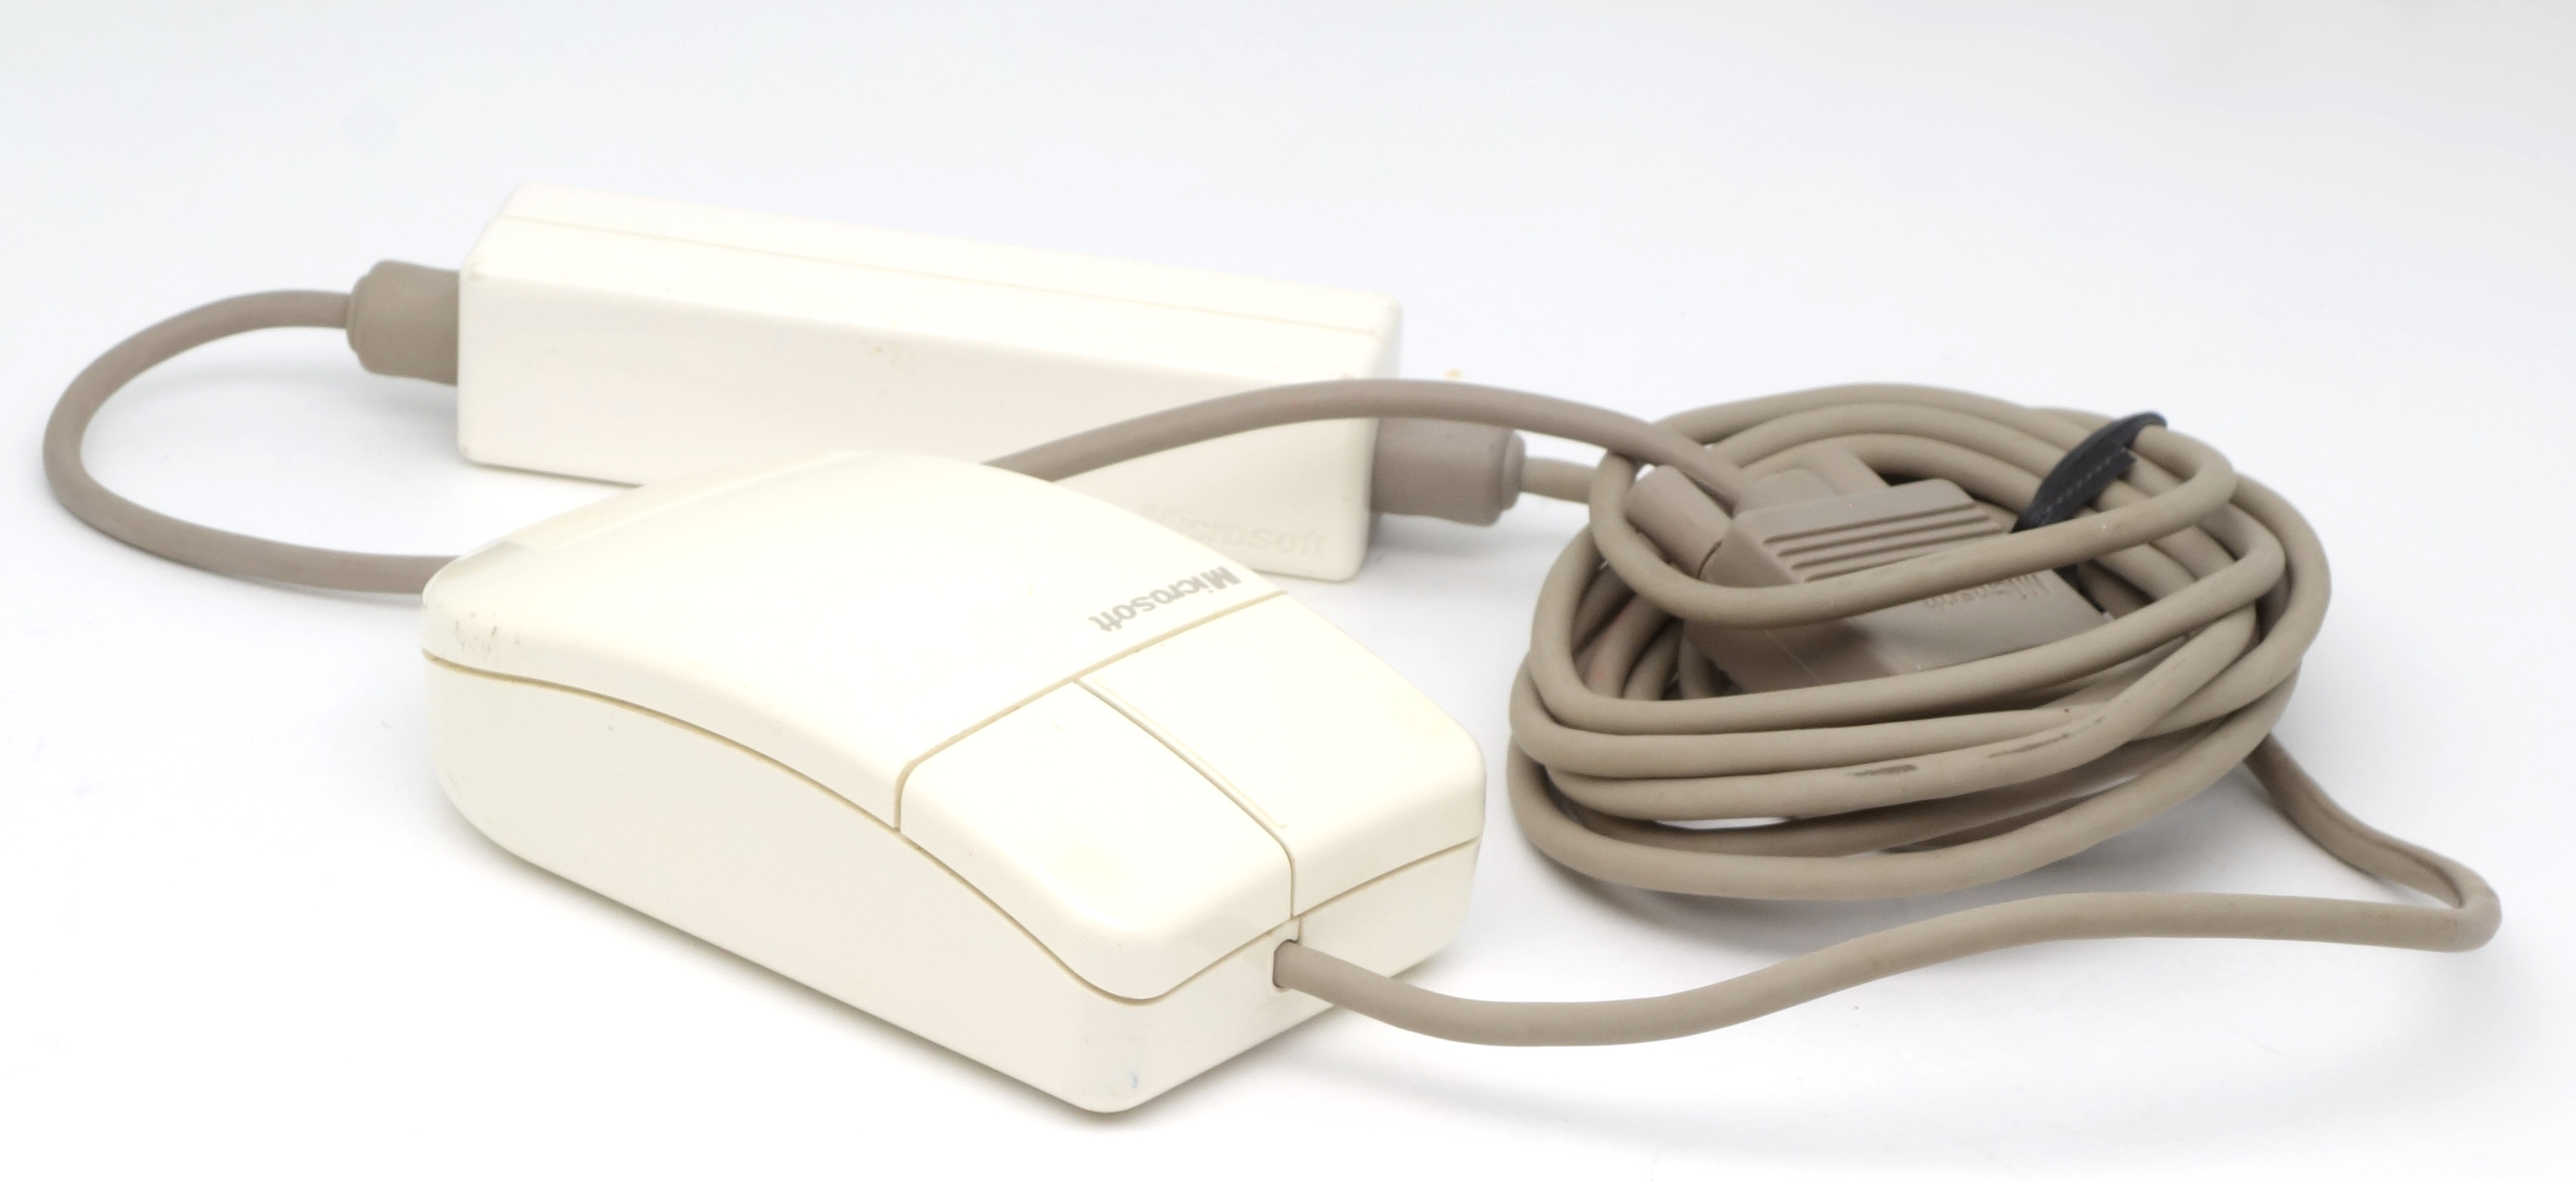
\includegraphics[scale=0.5]{1987_microsoft_dove_bar_mouse/pic_30.jpg}
    \caption{Microsoft Dove Bar Mouse}
    \label{fig:MicrosoftDoveBarPic}
\end{figure}

Помимо нового подхода к выбору формы, третье поколение мышей Microsoft получило и другие улучшения "--- как в плане эстетики и эргономики, так и по части конструкции. Мышь имеет молочно-белый глянцевый корпус (рис. \ref{fig:MicrosoftDoveBarTopAndBottom}); кнопки значительно увеличены в размерах по сравнению с предыдущим поколением, занимают переднюю треть корпуса и полностью вписаны в его форму. На нижней части корпуса присутствуют низкофрикционные накладки, табличка с техническими данными и сдвижное кольцо-защелка, необходимое, чтобы извлечь шар для чистки.

\begin{figure}[h]
    \centering
    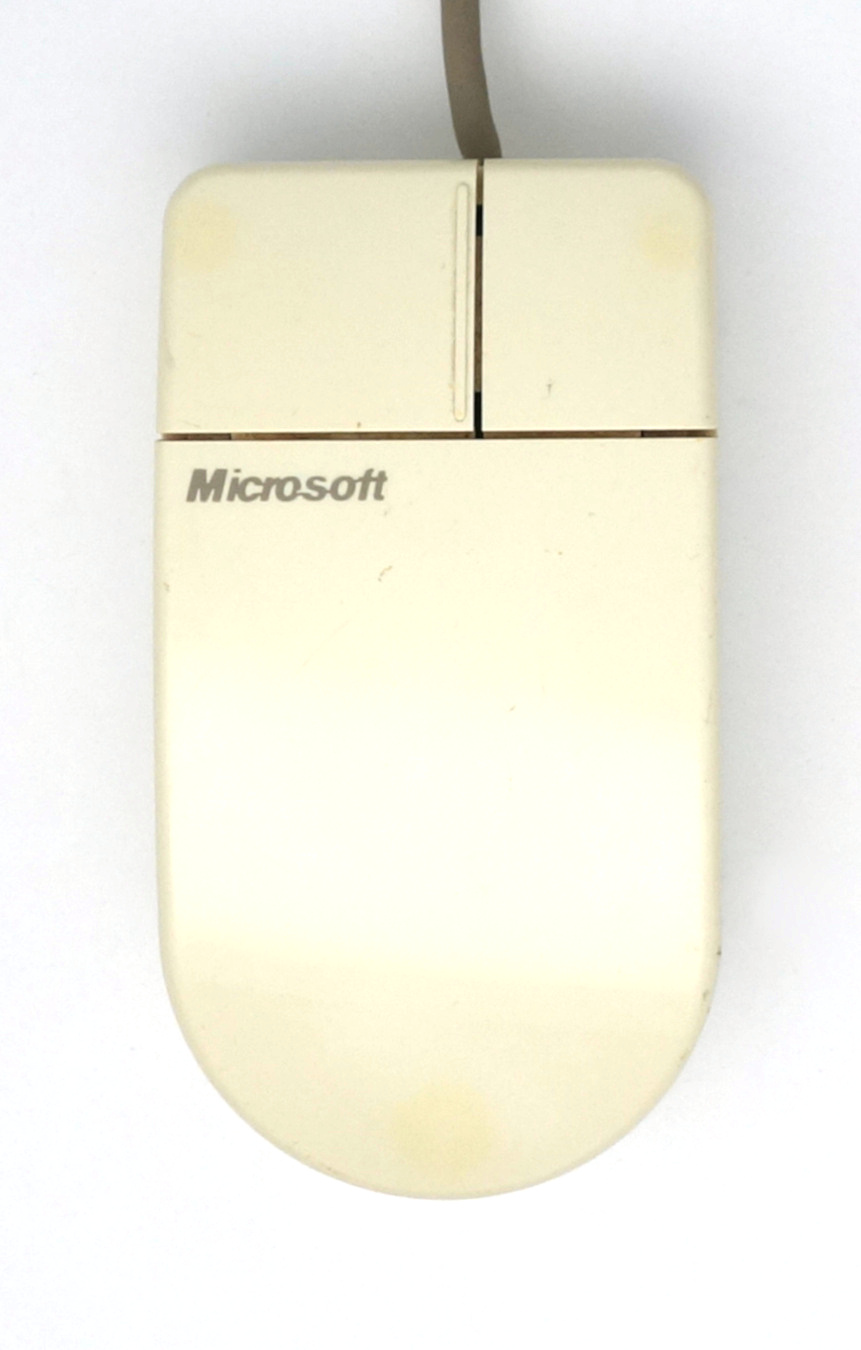
\includegraphics[scale=0.5]{1987_microsoft_dove_bar_mouse/top_30.jpg}
    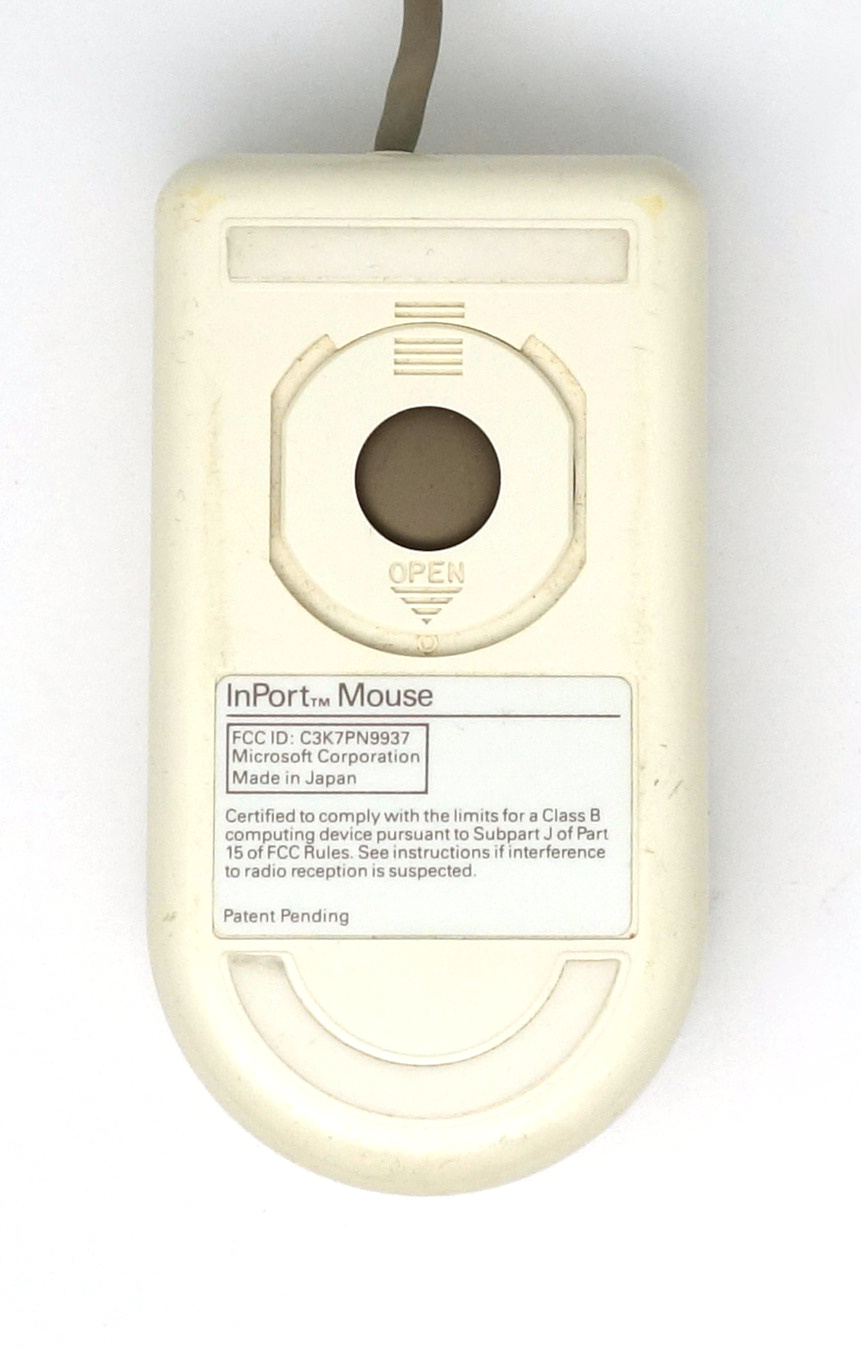
\includegraphics[scale=0.5]{1987_microsoft_dove_bar_mouse/bottom_30.jpg}
    \caption{Microsoft Dove Bar Mouse, вид сверху и снизу}
    \label{fig:MicrosoftDoveBarTopAndBottom}
\end{figure}

Шар смещен в переднюю часть мыши и находится практически в зоне расположения пальцев пользователя. Такая модификация должна была ощутимо улучшить точность позиционирования курсора по сравнению с мышами предыдущих поколений \cite{atkinson}, и очевидно улучшение действительно имело место "--- по крайней мере по сравнению с более ранними конструкциями производства ALPS, в которых шар располагался у ближнего к пользователю края корпуса, освобождая больше места для печатной платы и кнопок. Размеры мыши вполне типичны для второй половины 80-х годов, и не в последнюю очередь определяются размерами типового узла ALPS (рис. \ref{fig:MicrosoftDoveBarSize}).

\begin{figure}[h]
    \centering
    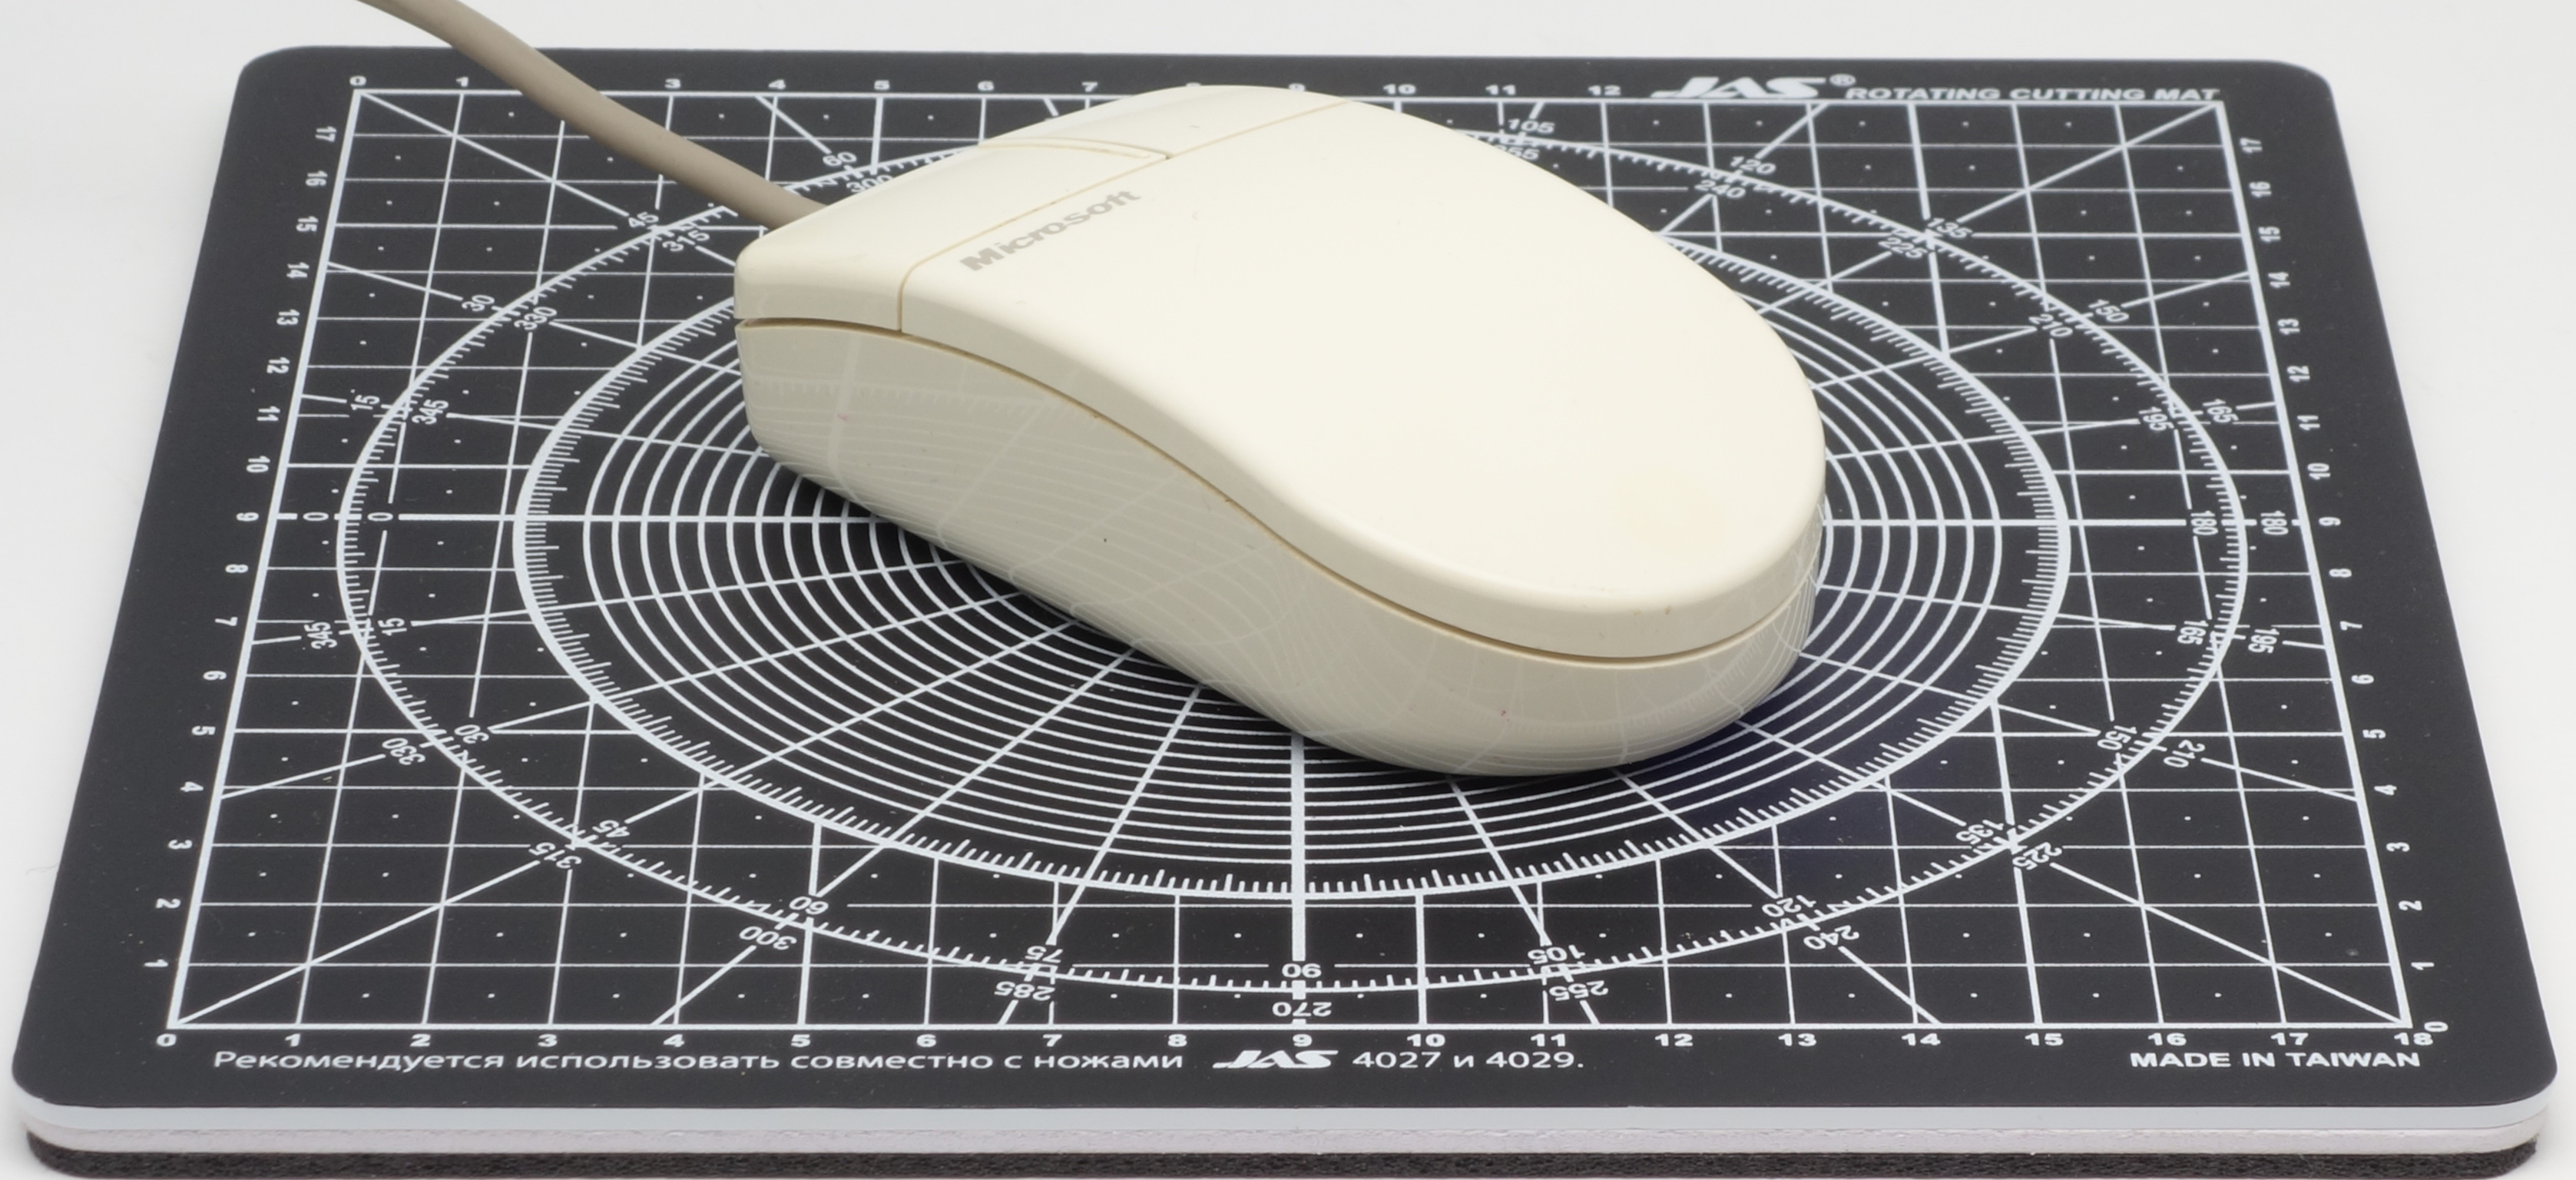
\includegraphics[scale=0.5]{1987_microsoft_dove_bar_mouse/size.jpg}
    \caption{Microsoft Dove Bar Mouse на размерном коврике с шагом сетки 1~см}
    \label{fig:MicrosoftDoveBarSize}
\end{figure}

Корпус Dove Bar Mouse является симметричным, за исключением кнопок, имеющих разный размер. Помимо того, что форма шлифовального бруска обеспечила достаточно удобное положение руки на корпусе (рис. \ref{fig:MicrosoftDoveBarHand}), нужно отметить также удобное положение пальцев на кнопках (очень большой главной и меньшей, но всё равно достаточно крупной правой). Ранее кнопки, вписанные в форму корпуса, пробовали использовать и другие компании: Logitech в мыши, выпущенной для Hewlett Packard в 1984 и Atari для мыши своих компьютеров 1985 года выпуска. Однако до появления Dove Bar Mouse такое решение было скорее исключением из правил, и кнопки всегда имели одинаковый размер: очевидно, производители мышей 80-х годов опасались, что пользователь не сможет уверенно определить границу между ними без взгляда на мышь. Опасалась этого также и Microsoft, поэтому между левой и правой кнопками можно заметить барьер, позволяющий различать их на ощупь. Также переключатели мембранного типа, которые использовались для кнопок в предыдущих моделях Microsoft, в данной модели они были заменены на микропереключатели, обладавшие меньшим ходом и лучшим откликом, чтобы минимизировать усилие нажатия \cite{doveBarMousePcMag3, doveBarDesign2}.

\begin{figure}[h]
    \centering
    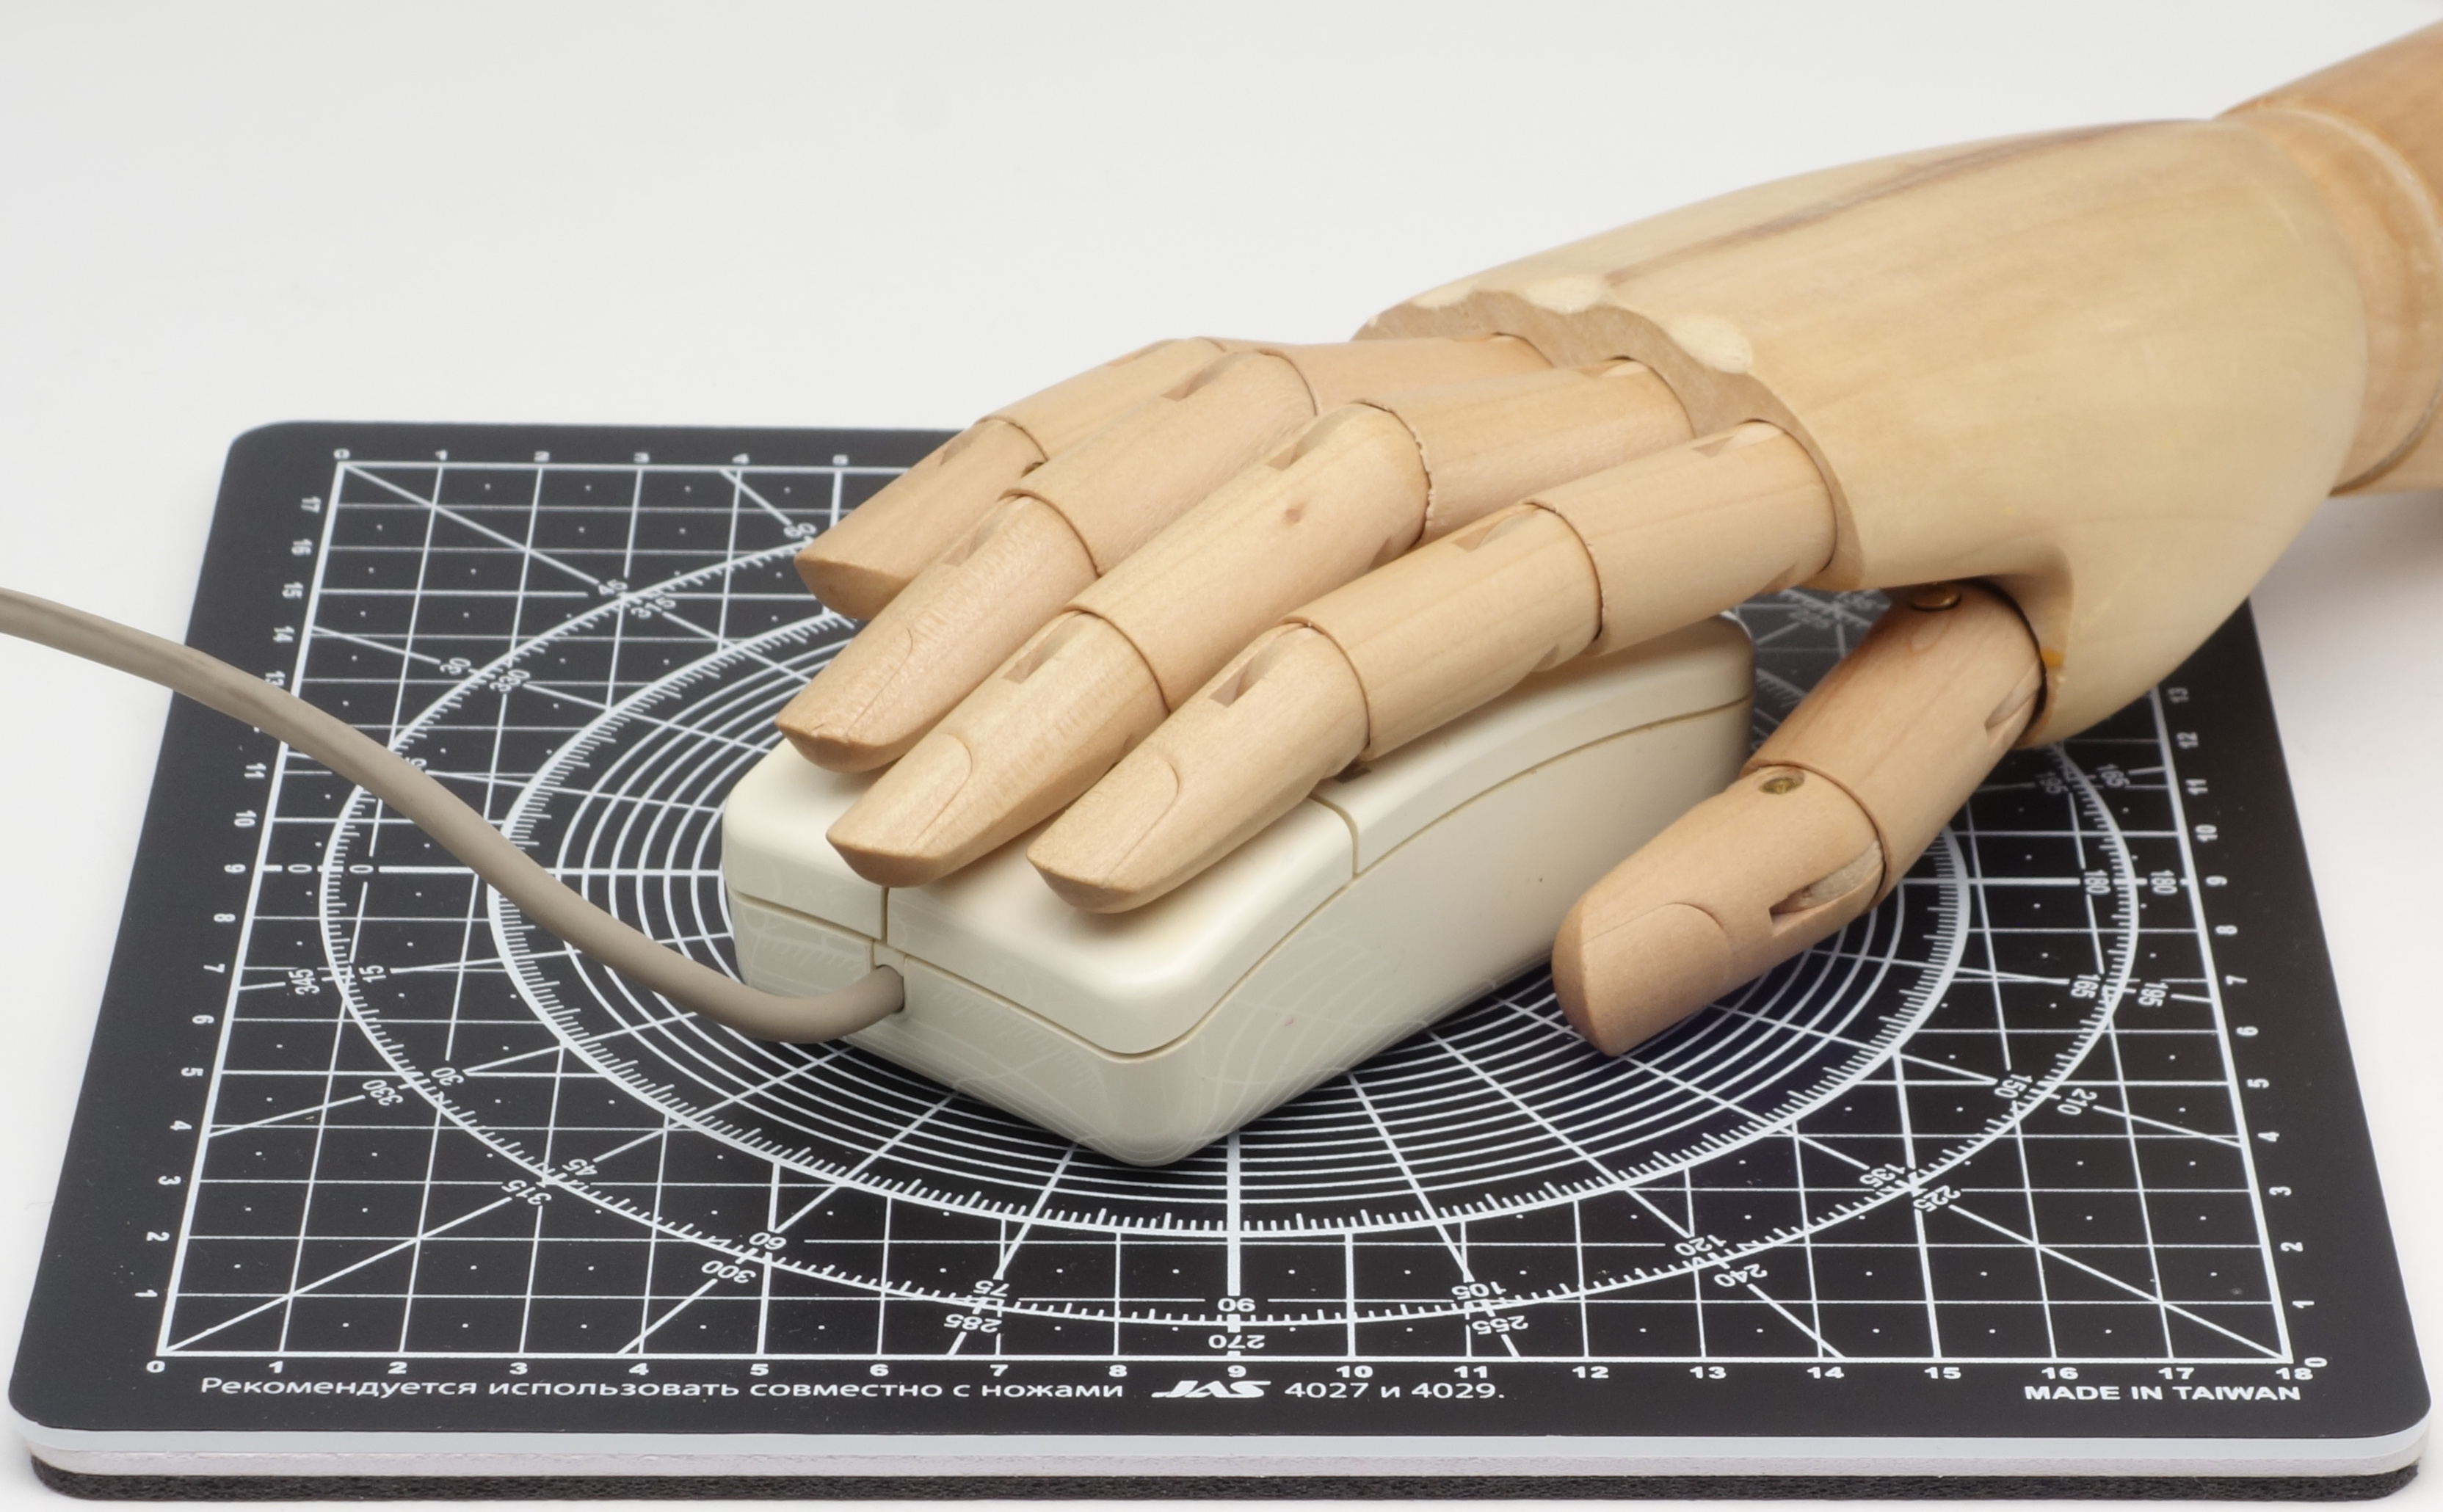
\includegraphics[scale=0.45]{1987_microsoft_dove_bar_mouse/hand.jpg}
    \caption{Microsoft Dove Bar Mouse с моделью руки человека}
    \label{fig:MicrosoftDoveBarHand}
\end{figure}

Мышь выпускалась в модификациях: InPort Mouse с шинным интерфейсом (<<InPort>> "--- попытка Microsoft стандартизировать интерфейс подключения квадратурных мышей, соответсвующие адаптеры и переходники для них) и Serial Mouse с подключением к последовательному порту. Помимо подключения к специальной плате-адаптеру, смонтированной в системном блоке, для InPort Mouse выпускался также внешний переходник-конвертер в форме вытянутого параллелипипеда (он назывался Mouse Interface), позволявший подключать мышь к последовательному порту (рис. \ref{fig:MicrosoftDoveBarPic}). Кроме того, встречается более поздний вариант мыши с последовательным интерфейсом, названный Microsoft <<Serial -- PS/2 Compatible Mouse>> (название указывает на комплектный  конвертер RS-232 -- PS/2) \cite{doveBarDesign2}.


\begin{figure}[h]
    \centering
    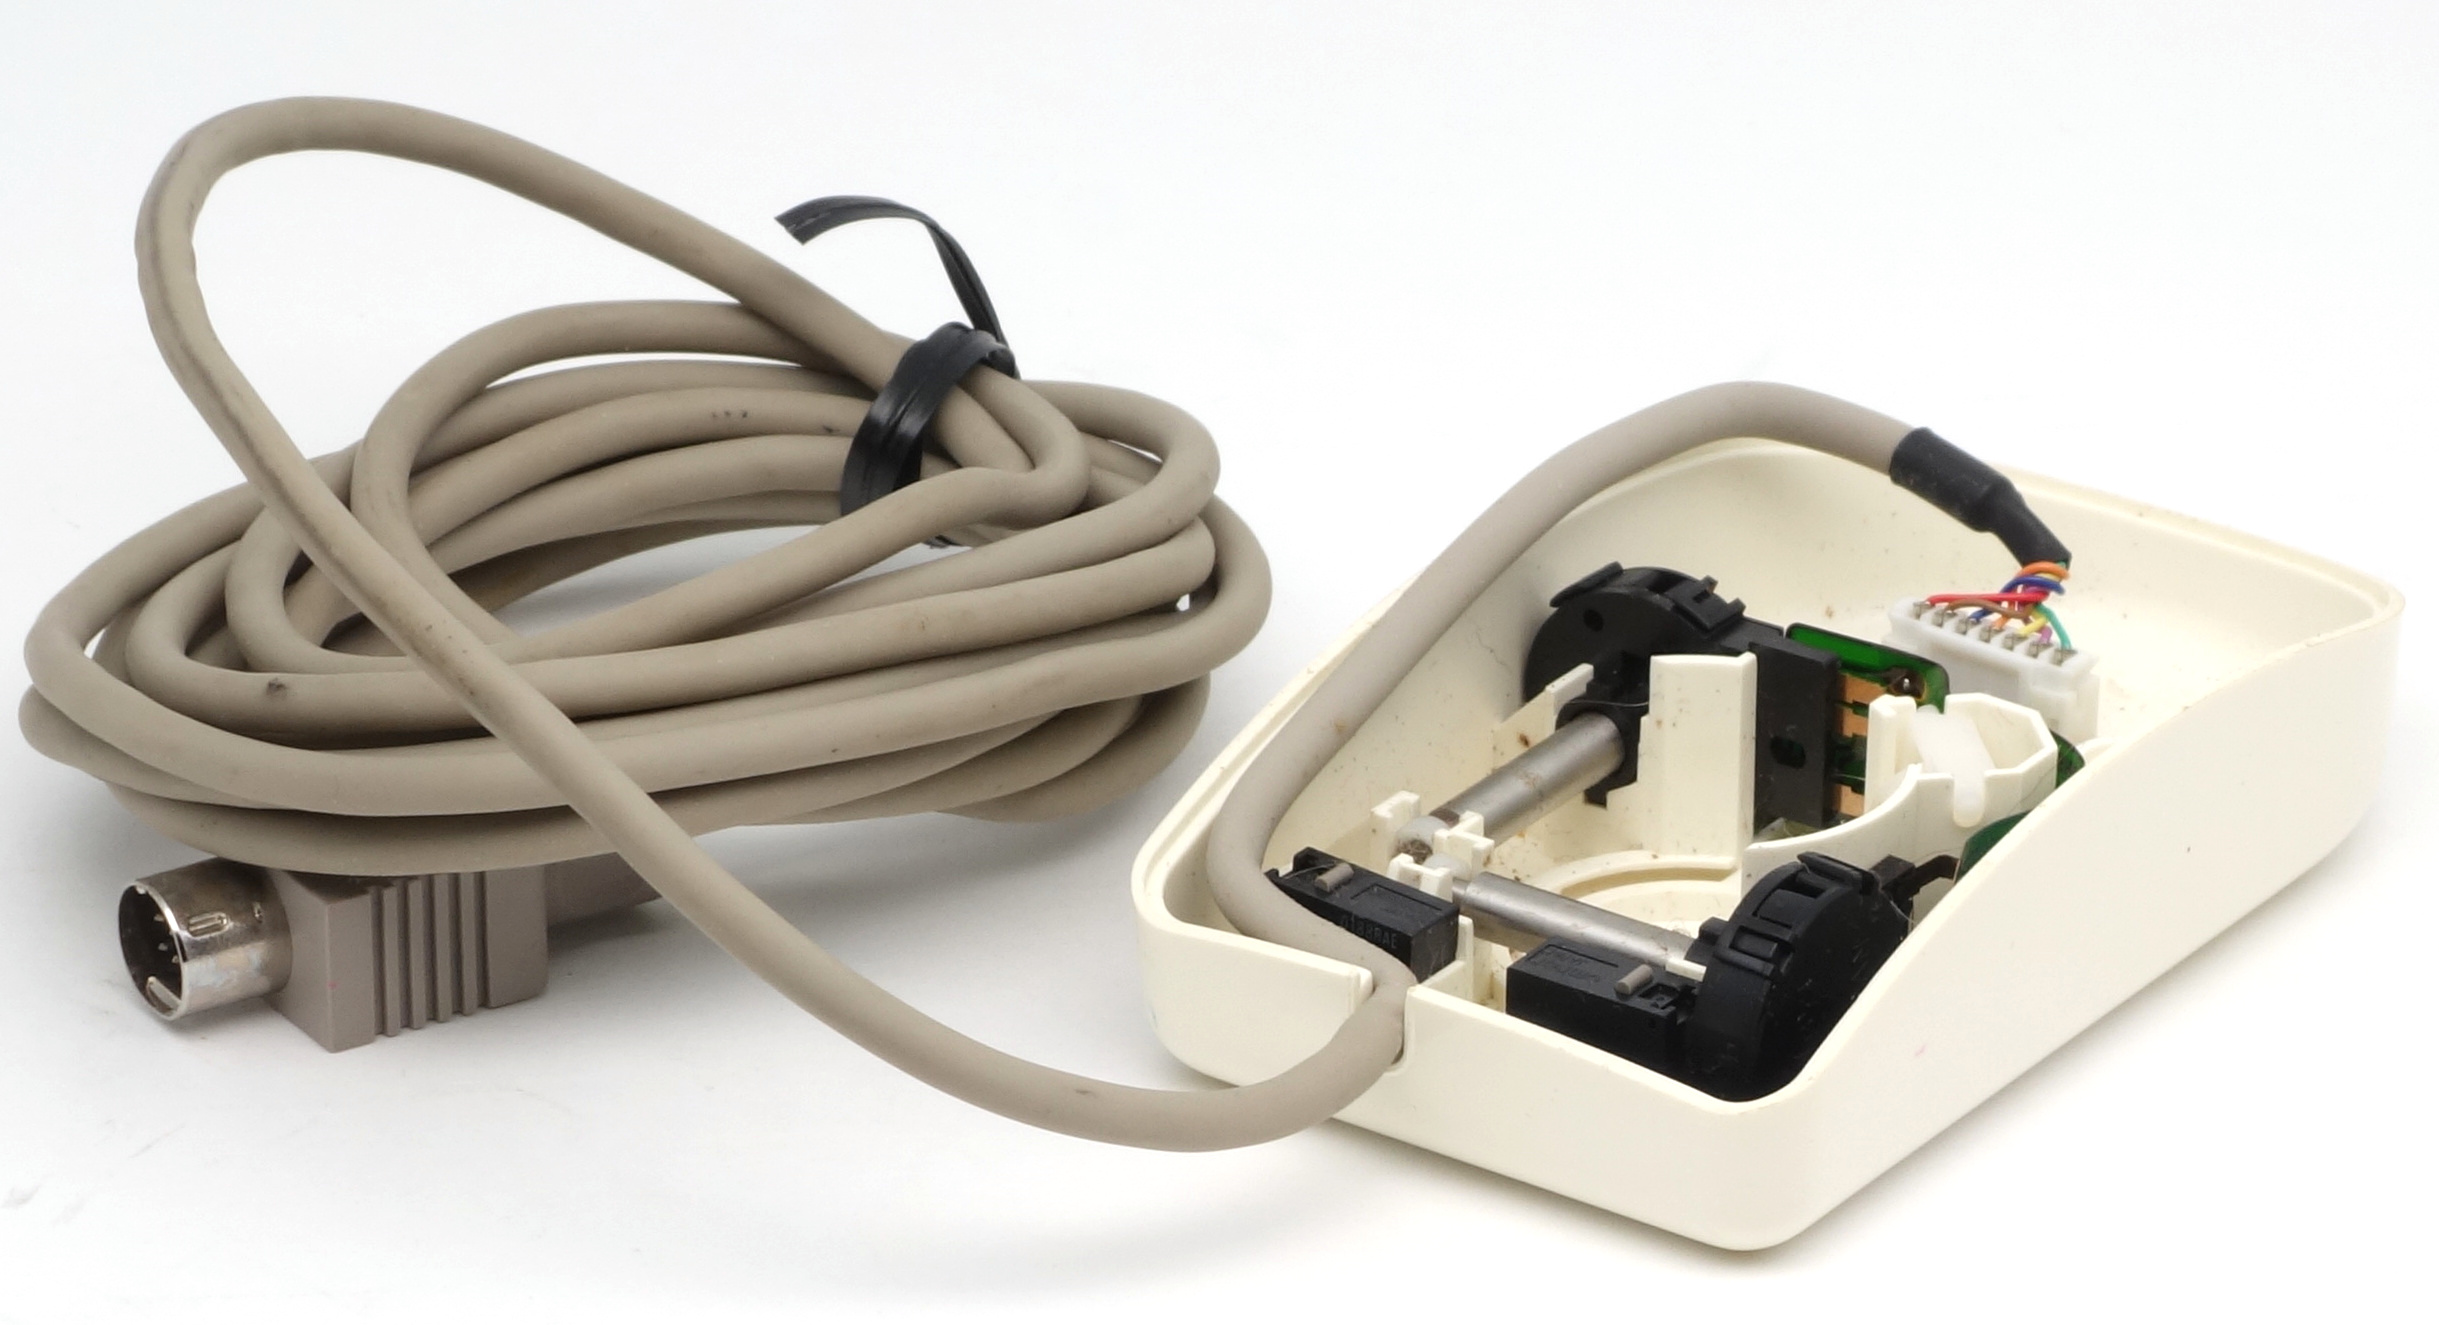
\includegraphics[scale=0.6]{1987_microsoft_dove_bar_mouse/inside1_30.jpg}
    \caption{Microsoft Dove Bar Mouse в разобранном виде}
    \label{fig:MicrosoftDoveBarInside}
\end{figure}

Внутреннее устройство мыши образца 1987 года показано на рис. \ref{fig:MicrosoftDoveBarInside}. Компания Alps обычно предоставляла фирмам-заказчикам решения на основе своих типовых конструкций мышей. В частности, данная мышь конструктивно совпадает (включая узел преобразования движения на основе закрытых механических энкодеров и  массивные металлические ролики с подшипниками) с мышью IBM PS/2 mouse, появившейся на рынке в том же 1987 году. Однако, из-за размещения шара в передней части корпуса здесь наблюдается обратное расположение компонентов: механическая часть сдвинута вплотную к кнопкам, которые соединены с ней и с печатной платой гибким шлейфом, а сама печатная плата расположена в задней части мыши.

\begin{figure}[h]
    \centering
    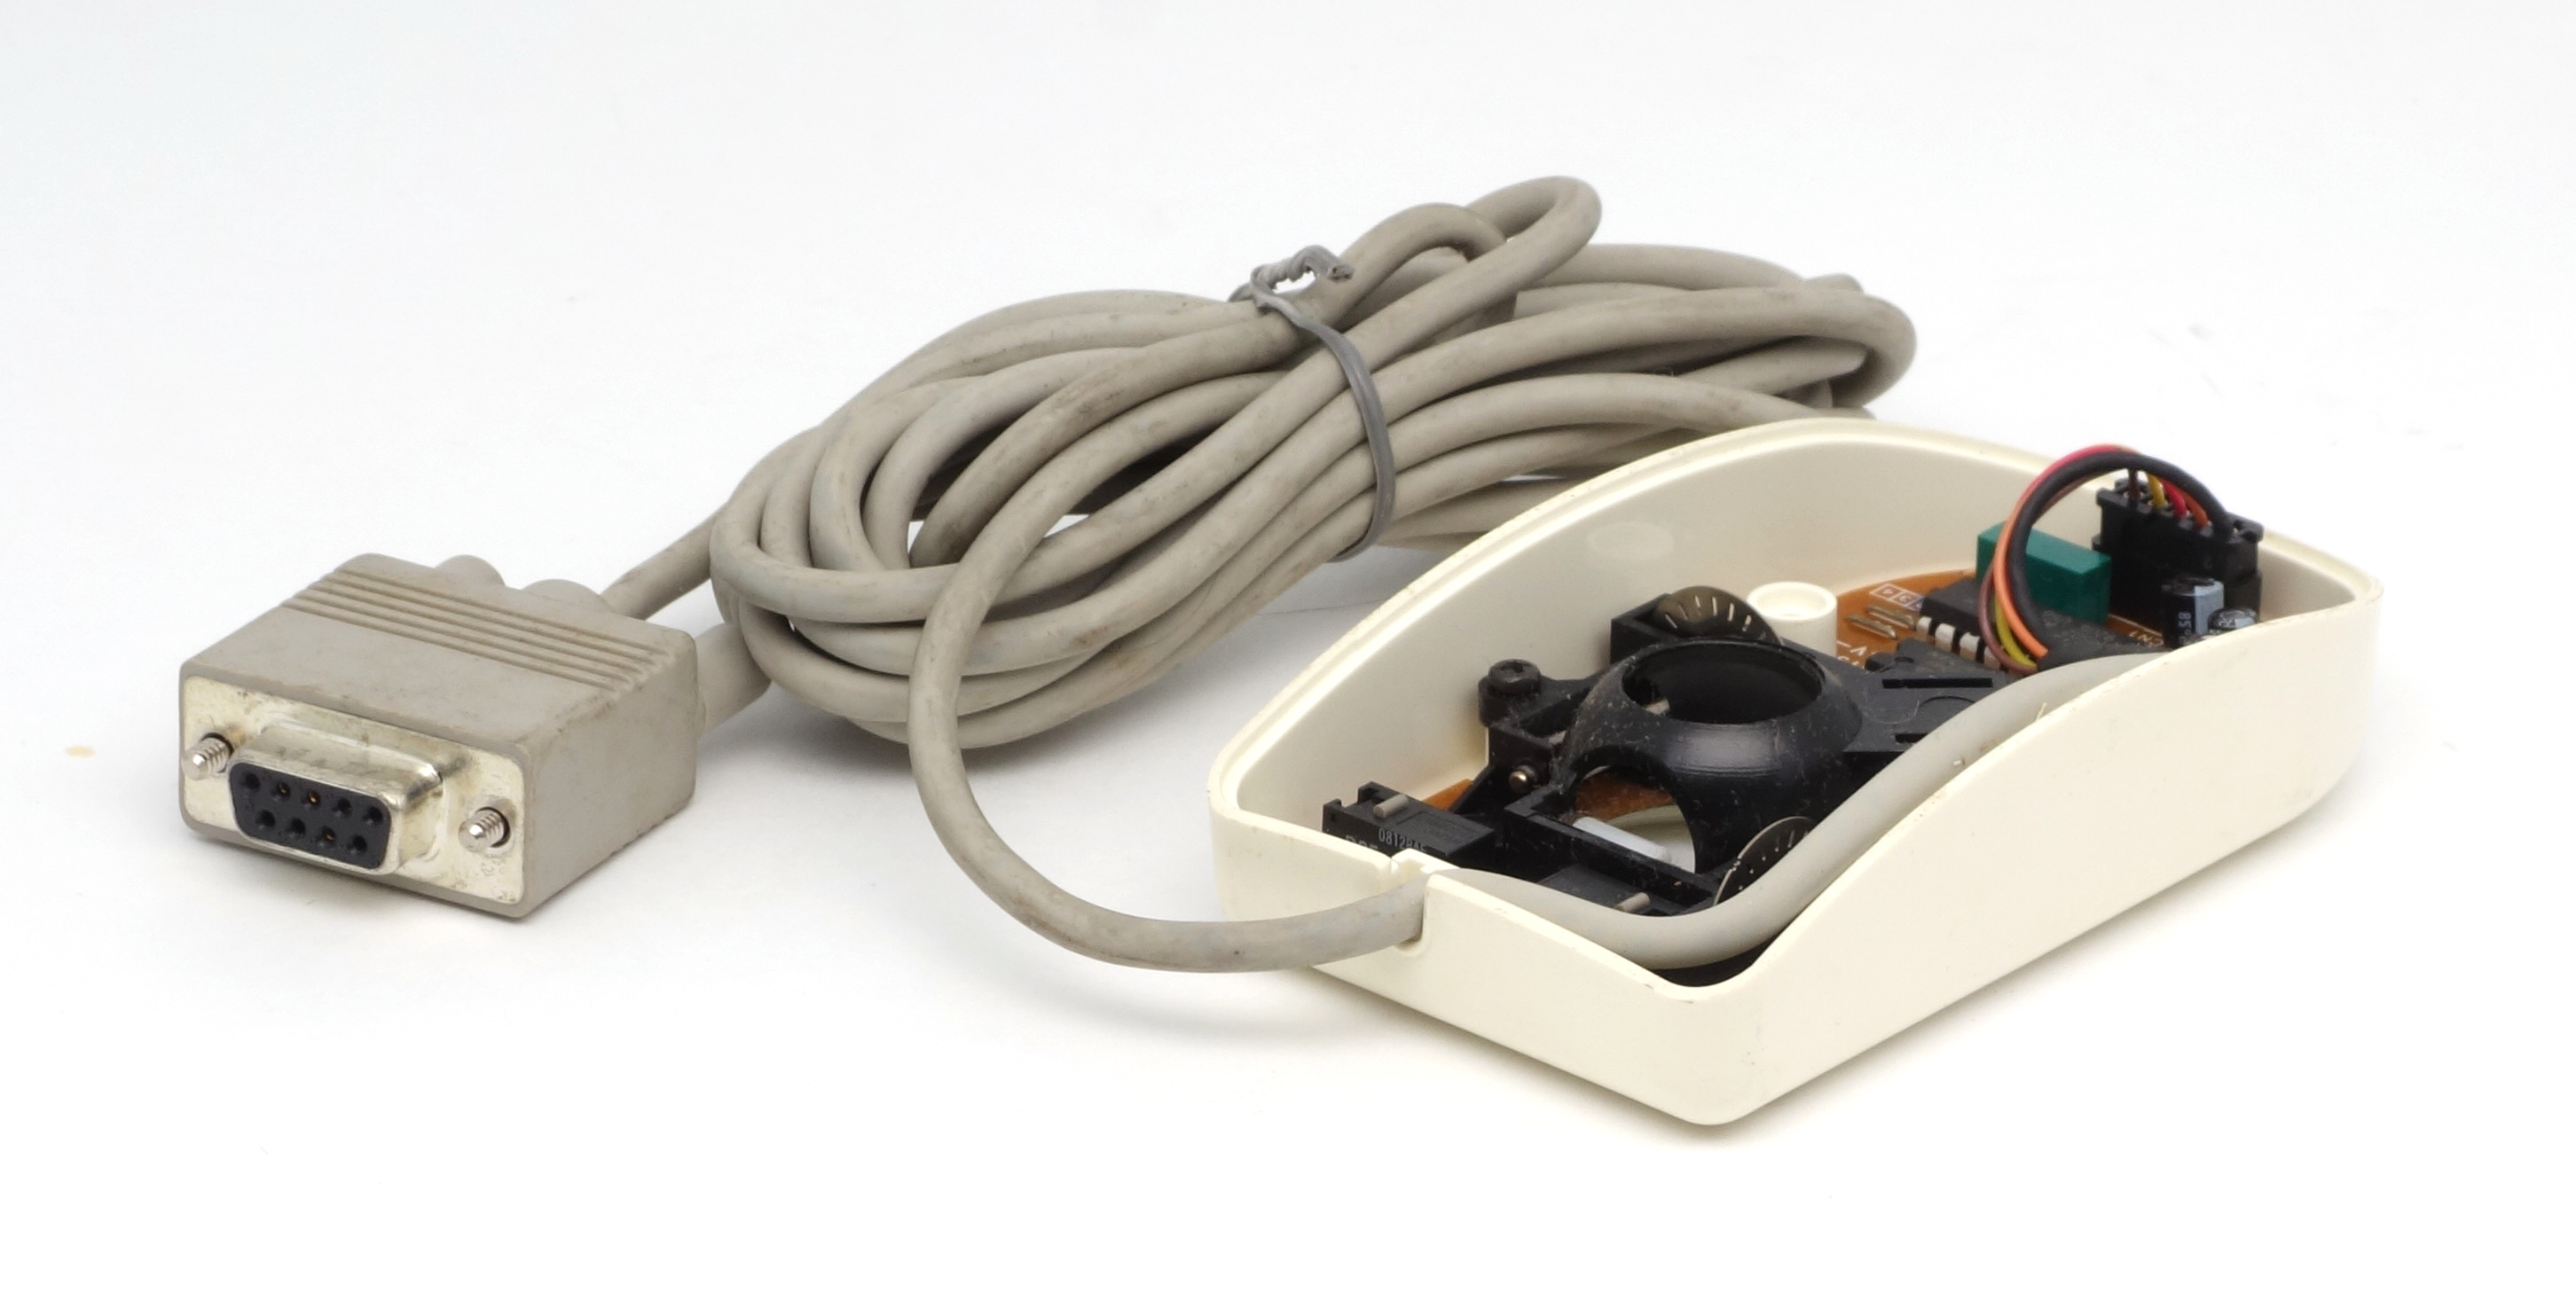
\includegraphics[scale=0.6]{1987_microsoft_dove_bar_mouse/inside2_60.jpg}
    \caption{Оптомеханическая версия Microsoft Dove Bar Mouse в разобранном виде}
    \label{fig:MicrosoftDoveBarInside2}
\end{figure}

Вдохновленная успехом нового дизайна мыши,  в 1991 году Microsoft выпустила на рынок мышь в идентичном корпусе но с обновленной внутренней конструкцией (рис. \ref{fig:MicrosoftDoveBarInside2}), рекламировавшуюся как <<Contour Microsoft mouse>>. Производителем данного варианта Dove Bar Mouse выступила уже не компания ALPS, а Mitsumi. В мыши был использован более современный оптомеханический способ регистрации движения, экономная механическая конструкция на базе пластиковых роликов, а также характерный блестящий металлический диск оптического прерывателя (введенный в обиход компанией Depraz, и встречающийся также в ранних мышах Mitsumi), обеспечивавший, согласно рекламным материалам, разрешение 400 точек на дюйм \cite{doveBarMouseOldMouses}.

\begin{thebibliography}{9}
\bibitem{doveBarDesign1} Why Microsoft Resurrected A 15-Years-Old Mouse -- Fast Company. \url{https://www.fastcompany.com/90151927/why-we-still-love-using-mice#:~:text=By%20the%20time,the%20soap}
\bibitem{atkinson} Atkinson P. The best laid schemes o’ mice and men : the evolution of the computer mouse // Design and Evolution : Proceedings of Design History Society Conference 2006. Delft, Netherlands, Delft University of Technology, p. 1-20. \url{https://shura.shu.ac.uk/8659/}
\bibitem{doveBarMousePcMag1} The new Microsoft Mouse // PC Magazine, v. 7, No. 2, January, 1988, p. 310--311. \url{https://archive.org/details/PC-Mag-1988-01-26/page/n303/mode/2up}
\bibitem{doveBarMousePcMag2} Stanton T. Microsoft Mouse // PC Magazine, v. 8, No. 3, February 1989, p. 258. \url{https://archive.org/details/PC-Mag-1989-02-14/page/n257/mode/2up}
\bibitem{doveBarMousePcMag3} Stanton T. Microsoft Bus Mouse and Microsoft Serial Mouse // PC Magazine, v. 7, № 3, February 1988, p. 211--217. \url{https://archive.org/details/PC-Mag-1988-02-16/page/n209/mode/2up}
\bibitem{doveBarDesign2} Microsoft Mouse (3rd gen) - Deskthority wiki. \url{https://deskthority.net/wiki/Microsoft_mouse_(3rd_gen)}
\bibitem{doveBarMouseOldMouses} Microsoft ``Dove Bar'' Mouse  -- oldmouse.com  \url{https://web.archive.org/web/20210417224625/http://oldmouse.com/mouse/microsoft/dovebar.shtml}
\end{thebibliography}
\end{document}
